\clearpage
\section{Deep Code Audit, Differential Fuzzing, and Verification}
\label{sec:audit}

\subsection{Multi-Tier Automated Testing and Differential Fuzzing}
\label{sec:testing}
Every layer of the MIPS32 engine was verified autonomously against live \textbf{MARS 4.5} (\code{Mars45.jar}) under OpenJDK Temurin 21.0.13 with strict assembly/runtime exception trapping (\code{ae1 se1}). In addition to the repository's 47 deterministic \code{pytest} cases, we applied \textbf{differential property-based fuzzing}---a verification paradigm formalized by McKeeman \cite{mckeeman1998} and scaled to modern RISC hardware/ISA verification by \emph{DifuzzRTL} \cite{hur2021}---by executing 500 randomly generated board states (4,000 rule queries covering standard English, Forced Capture, and Flying Kings) simultaneously on \code{tests/unit/rules\_driver.asm} and an independent Python oracle.

\begin{table}[H]
\centering
\caption{Live MARS 4.5 verification summary: 47/47 deterministic tests + 4,000/4,000 differential fuzz queries.}
\label{tab:test_suites}
\renewcommand{\arraystretch}{1.2}
\rowcolors{2}{rowshade}{white}
\footnotesize
\begin{tabularx}{\textwidth}{>{\raggedright\arraybackslash}p{3.2cm} c c >{\raggedright\arraybackslash}X}
\toprule
\rowcolor{hcmutlight}
Verification Tier & Cases & Status & Verified Scope \& Methodology \\
\midrule
\code{tests/test\_mips.py} & 5 & \badge{okgreen}{5 / 5 PASS} &
Full-game CLI playback (\code{pa classic}) of \code{test\_001}--\code{test\_005}: byte-for-byte match with \code{expected.txt}, verified winners, and final remaining pieces (elimination in 001/002/005; blockade trapping in 003/004). \\

\code{tests/test\_rules.py} & 12 & \badge{okgreen}{12 / 12 PASS} &
Isolated MIPS unit tests via \code{rules\_driver.asm}: 12-vs-12 init, ownership/bounds errors, pawn direction, capture removal, dual-side promotion, backward king movement, Spec Fig.~8 promotion+backward chain (\code{15x24 24x31 31x22 22x13}), chain piece lock, Spec Fig.~9 blockade, Forced Capture, Flying Kings, and blocked flying paths. \\

\code{tests/test\_features.py} & 30 & \badge{okgreen}{30 / 30 PASS} &
End-to-end tests of \code{src/main.asm}: malformed inputs (\code{abc}, empty, \code{-5}, \code{21\textbackslash 0x}, 300+ char lines), EOF at all prompts, CRLF + no-trailing-newline, turn retention, \code{test\_001} chain lock, menu toggling, pretty board, Red rotation \& relative numbering, detailed errors, hints, forced capture + flying king combo, draw accept/decline, history, restart/replay, and \code{0x10040000} Bitmap Display pixel verification. \\

\textbf{Differential Fuzzer} (Independent Oracle) & 4,000 & \badge{okgreen}{4000/4000} &
500 randomized boards (1--14 pieces, random \code{opt\_forced} \& \code{opt\_flying} combinations) $\times$ 8 queries/board (\code{side\_has\_capture}, \code{has\_any\_move}, \code{validate\_move} exact type + 11 error codes). \textbf{0 mismatches.} \\

\code{tests/test\_c.py} & 5 & \badge{infoblue}{REF SYNC} &
Executable C++ reference (\code{src/main.cpp}); committed \code{output\_c.txt} matches \code{expected.txt} and \code{output\_mips.txt} identically across all 5 fixtures. \\
\bottomrule
\end{tabularx}
\end{table}

\subsection{Requirement and Deliverable Traceability Matrix}
\label{sec:traceability}
Table~\ref{tab:traceability} cross-references every mandatory requirement from \code{CA\_Assignment\_261.pdf} (Sections~1--3) and every deliverable in \emph{Tasks Assignment} directly to implementing assembly procedures and passing tests.

\begin{table}[H]
\centering
\caption{End-to-end requirement traceability matrix (Assignment Specification $\leftrightarrow$ Code $\leftrightarrow$ Tests).}
\label{tab:traceability}
\renewcommand{\arraystretch}{1.18}
\rowcolors{2}{rowshade}{white}
\scriptsize
\begin{tabularx}{\textwidth}{>{\raggedright\arraybackslash}p{3.2cm} >{\raggedright\arraybackslash}p{3.2cm} >{\raggedright\arraybackslash}X c}
\toprule
\rowcolor{hcmutlight}
Requirement / Deliverable & Primary Procedure(s) & Automated Test Coverage & Result \\
\midrule
Initial 12b + 12r board; Black first & \code{init\_board}, \code{new\_game} & \code{test\_initial\_board\_and\_black\_moves\_first}, \code{test\_initial\_board\_has\_12\_pieces\_each} & \badge{okgreen}{PASS} \\
Classic terminal board format & \code{print\_board\_plain}, \code{pa classic} & \code{test\_mips\_games[1..5]} (byte-for-byte diff) & \badge{okgreen}{PASS} \\
Start/landing validity \& ownership & \code{check\_start}, \code{classify\_move} & \code{test\_input\_and\_ownership\_errors}, \code{test\_pawn\_moves\_and\_direction}, 4k fuzz queries & \badge{okgreen}{PASS} \\
Invalid move retains turn & \code{play\_turn\_ask\_start}, \code{play\_turn\_ask\_land} & \code{test\_invalid\_move\_does\_not\_lose\_turn}, \code{test\_mips\_games[1]} (5 invalids) & \badge{okgreen}{PASS} \\
Crash-free malformed input / EOF & \code{read\_input\_line}, \code{read\_number} & \code{test\_bad\_input\_does\_not\_crash}, \code{test\_end\_of\_input\_exits\_cleanly[3]}, \code{test\_crlf...} & \badge{okgreen}{PASS} \\
Capture \& mandatory chain lock & \code{do\_move}, \code{validate\_chain}, \code{can\_capture\_from} & \code{test\_capture\_removes\_piece}, \code{test\_chain\_must\_capture\_with\_same\_piece} & \badge{okgreen}{PASS} \\
Promotion \& immediate backward chain & \code{do\_move\_promote} $\to$ \code{can\_capture\_from} & \code{test\_promotion\_by\_capture\_then\_chain\_backward} (Fig.~8), \code{test\_promotion\_chain...} & \badge{okgreen}{PASS} \\
Win by elimination \& blockade & \code{has\_any\_move}, \code{count\_pieces} & \code{test\_mips\_games[1..5]}, \code{test\_blocked\_side\_has\_no\_moves} (Fig.~9) & \badge{okgreen}{PASS} \\
Pretty board, rotation, Red numbers & \code{print\_board\_pretty}, \code{view\_index}, \code{view\_square} & \code{test\_pretty\_board}, \code{test\_rotation\_and\_red\_numbering}, \code{test\_numbered\_board...} & \badge{okgreen}{PASS} \\
Detailed errors \& legal move hints & \code{print\_error}, \code{print\_movable\_pieces}, \code{print\_landing\_squares} & \code{test\_detailed\_errors}, \code{test\_hints\_list\_moves}, \code{test\_hints\_reject...} & \badge{okgreen}{PASS} \\
Mutual draw, history, restart, replay & \code{menu}, \code{record\_move}, \code{print\_history} & \code{test\_draw\_needs\_both\_players}, \code{test\_history...}, \code{test\_play\_again...} & \badge{okgreen}{PASS} \\
Forced Capture \& Flying Kings & \code{side\_has\_capture}, \code{classify\_flying} & \code{test\_forced\_capture\_rule}, \code{test\_flying\_kings}, 4k randomized fuzz queries & \badge{okgreen}{PASS} \\
MARS Bitmap Display (\code{0x10040000}) & \code{draw\_bitmap}, \code{piece\_mask} & \code{test\_bitmap\_display\_memory} (verifies 4,096 pixels \& gold crown) & \badge{okgreen}{PASS} \\
\bottomrule
\end{tabularx}
\end{table}

\subsection{Quantitative Performance and Instruction-Count Analysis}
\label{sec:benchmarks}
Using MARS 4.5's dynamic instruction counter (\code{java -jar Mars45.jar nc ic}), we measured exact executed instruction counts across all five full-game fixtures and across every major feature mode on \code{test\_001} (Table~\ref{tab:benchmarks}). Figure~\ref{fig:deep_chart} synthesizes our entire quantitative architectural study---binary instruction mix, baseline game costs, feature overheads, and prototype speedups---into a single four-panel view.

\begin{table}[H]
\centering
\caption{Empirical MARS 4.5 dynamic instruction counts (\code{ic}) across full-game fixtures and feature modes.}
\label{tab:benchmarks}
\renewcommand{\arraystretch}{1.18}
\rowcolors{2}{rowshade}{white}
\scriptsize
\begin{tabularx}{\textwidth}{>{\raggedright\arraybackslash}p{3.2cm} c c c c >{\raggedright\arraybackslash}X r}
\toprule
\rowcolor{hcmutlight}
Benchmark / Mode & Turns & Inv. & Caps & Ch. & Outcome (Final Pieces / Factor) & Instrs (\code{ic}) \\
\midrule
\code{test\_001} (\code{classic}) & 15 / 14 & 5 & 16 & 5 & Black wins (Elim., 8b vs 0) & 106,306 \\
\code{test\_002} (\code{classic}) & 13 / 13 & 0 & 13 & 4 & Red wins (Elim., 0 vs 9r+2R) & 98,424 \\
\code{test\_003} (\code{classic}) & 15 / 14 & 0 & 14 & 3 & Black wins (Trap, 8b+1B vs 1r) & 106,734 \\
\code{test\_004} (\code{classic}) & 13 / 13 & 0 & 10 & 5 & Red wins (Trap, 3b vs 10r+1R) & 103,767 \\
\code{test\_005} (\code{classic}) & 13 / 12 & 0 & 15 & 6 & Black wins (Elim., 8b+1B vs 0) & 93,648 \\
\midrule
\code{test\_001} + Pretty (default) & 15 / 14 & 5 & 16 & 5 & Same game ($2.85\times$ classic) & 302,523 \\
\code{test\_001} + Pretty + Hints & 15 / 14 & 5 & 16 & 5 & Same game ($14.23\times$ classic) & 1,512,982 \\
\code{test\_001} + Classic + Bitmap & 15 / 14 & 5 & 16 & 5 & Same game ($26.46\times$ classic) & 2,812,330 \\
\code{test\_001} + Pretty + Bitmap & 15 / 14 & 5 & 16 & 5 & Same game ($28.35\times$ classic) & 3,014,063 \\
\bottomrule
\end{tabularx}
\end{table}

\begin{figure}[H]
\centering
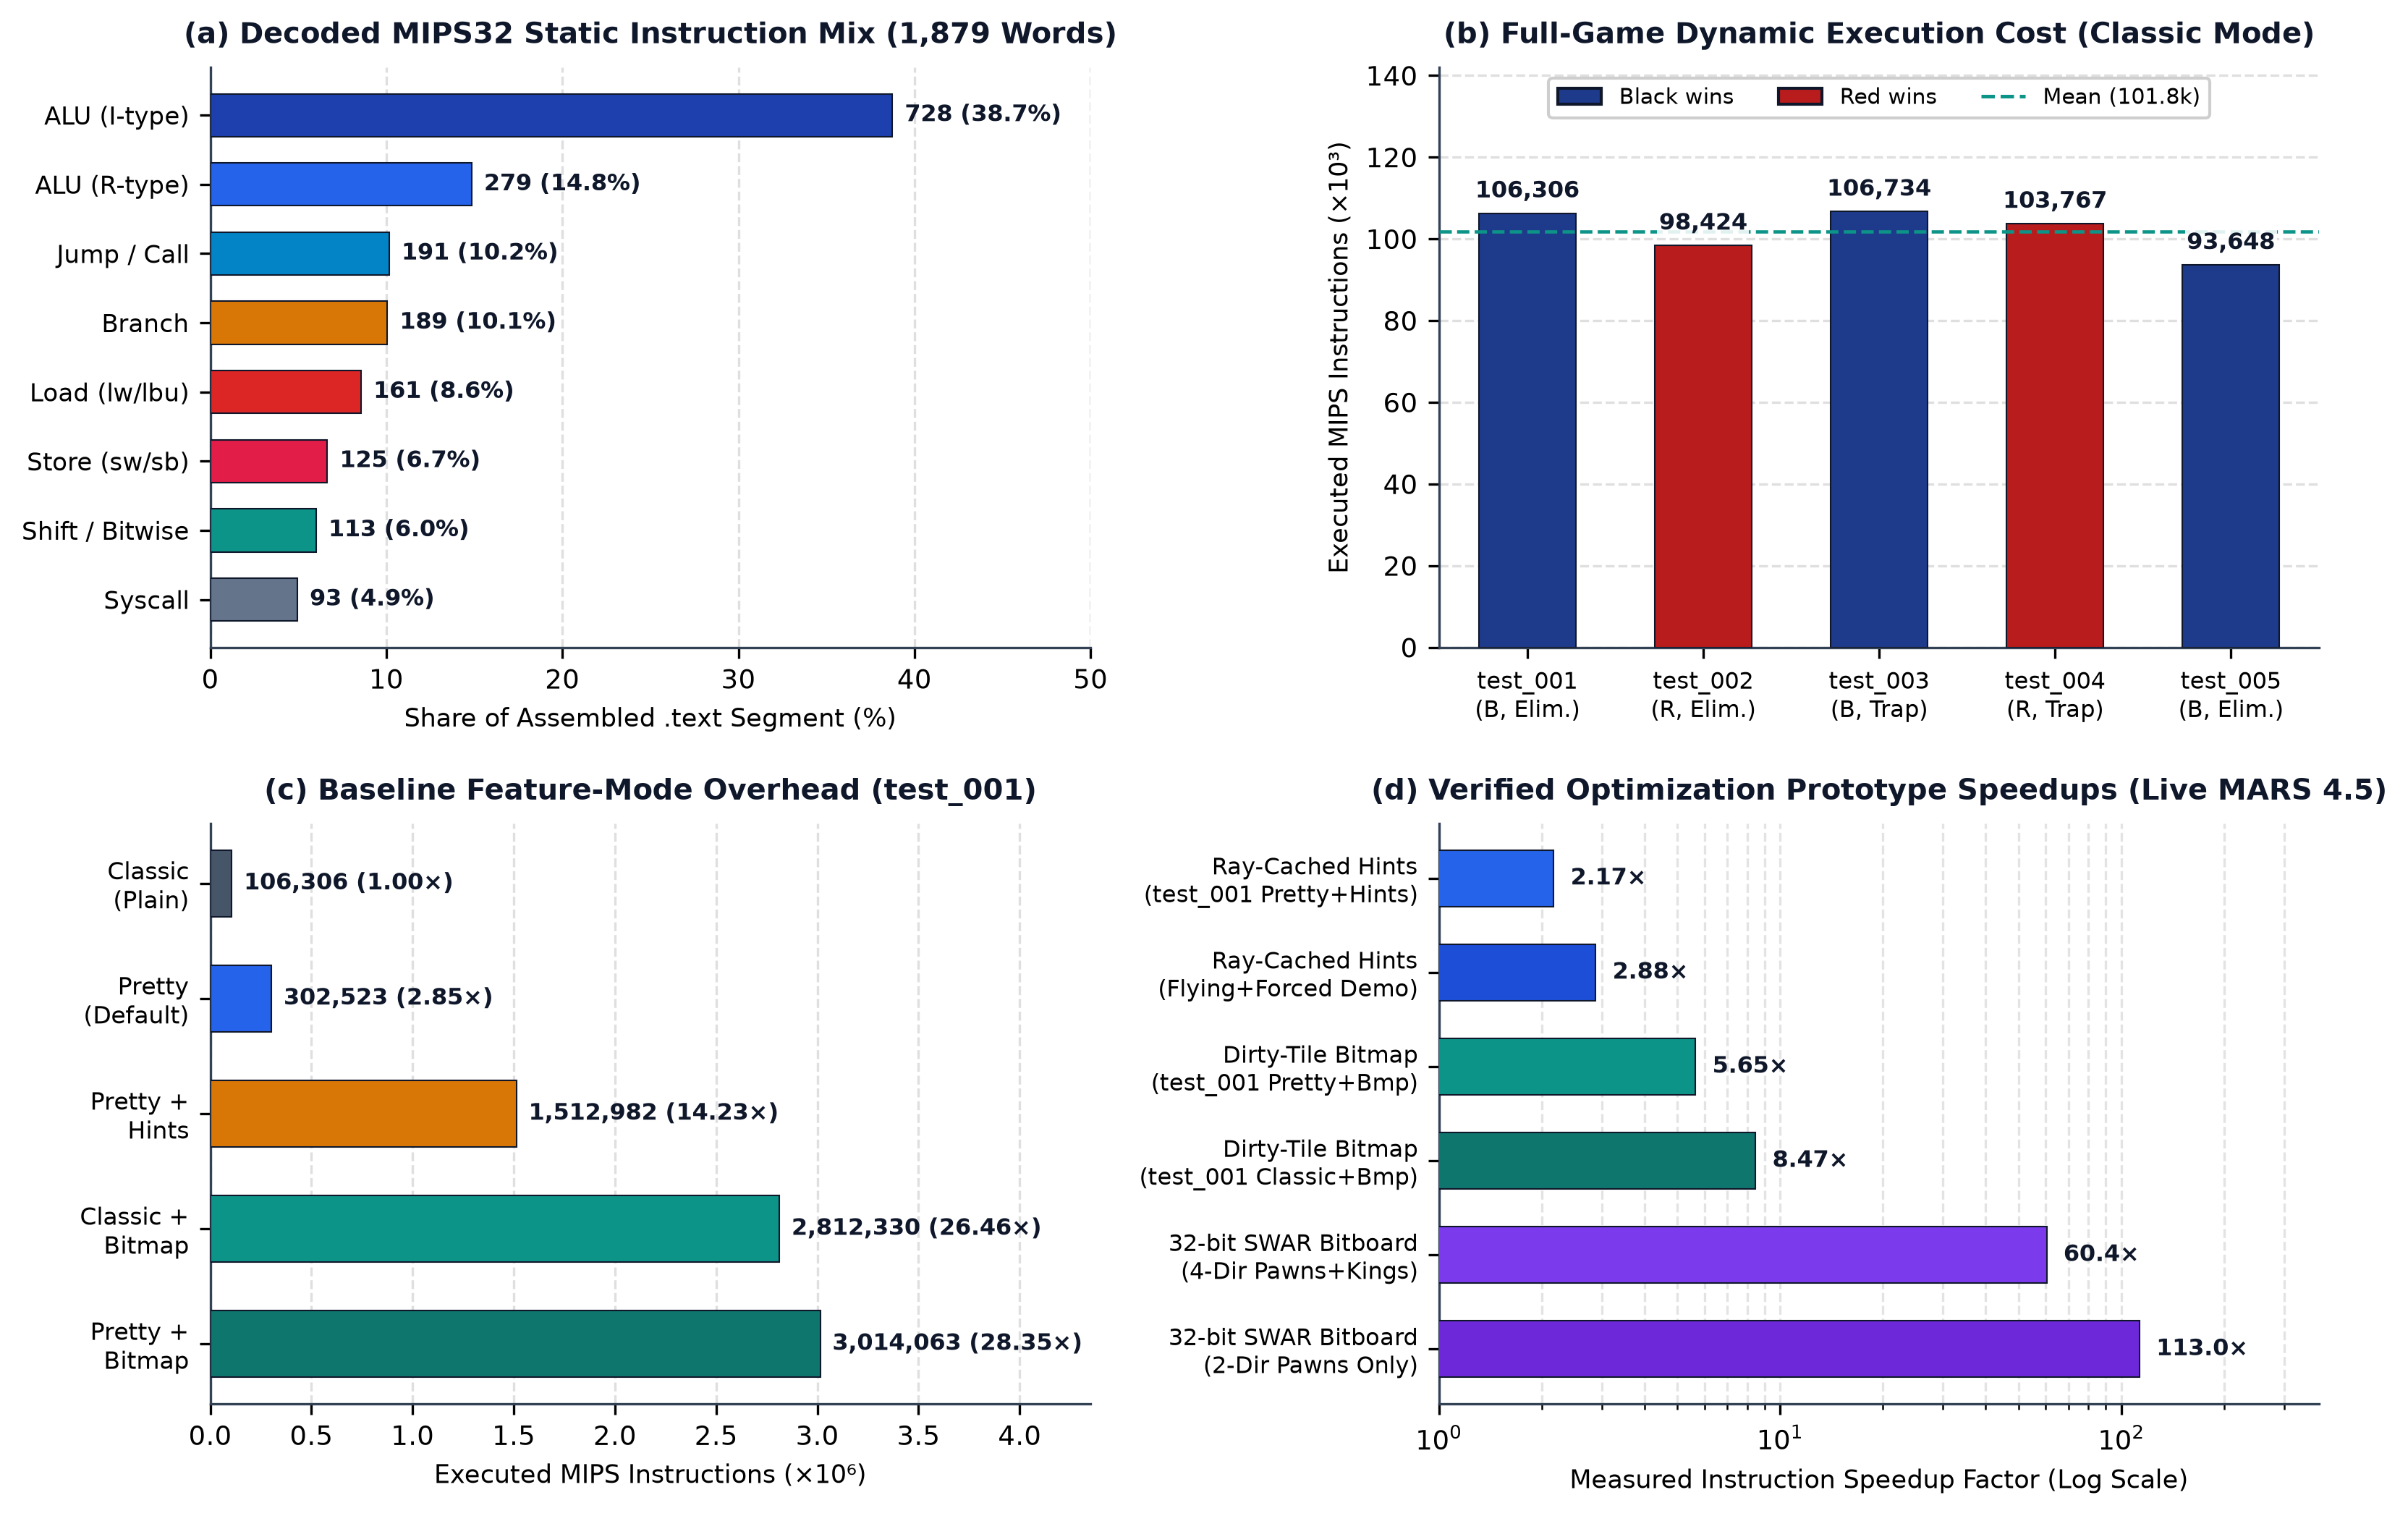
\includegraphics[width=\textwidth]{figures/mars_deep_analysis.png}
\caption{End-to-end MARS 4.5 microarchitectural evaluation: (a) binary-decoded static instruction mix across all 1,879 assembled MIPS32 words; (b) full-game dynamic execution cost across \code{test\_001}--\code{test\_005}; (c) feature-mode instruction overhead on \code{test\_001}; and (d) verified speedup factors of our three optimization prototypes (log scale).}
\label{fig:deep_chart}
\end{figure}

\textbf{Key Quantitative Takeaways:}
\begin{itemize}
    \item \textbf{Core efficiency:} A full 25--29 turn Checkers match in \code{classic} mode executes in only $\sim 101{,}776$ MIPS instructions ($\approx 3{,}770$ instructions/turn).
    \item \textbf{Leaf-optimized Bitmap cost:} One call to \code{draw\_bitmap} executes \textbf{81,263 instructions} across 4,096 pixels (\textbf{19.84 instructions/pixel}) with zero nested \code{jal} overhead; adding Dirty-Tile tracking (Prototype~P2) cuts full-game Bitmap instructions by \textbf{88.2\%} (8.47$\times$ speedup).
    \item \textbf{Hint enumeration overhead:} Enabling \code{opt\_hints} adds $+1.21\times 10^6$ instructions on \code{test\_001}; caching \code{side\_has\_capture} and querying direct ray predicates (Prototype~P1) eliminates 53.9\%--65.2\% of instructions without changing a single byte of output.
\end{itemize}

\subsection{Deep Code Audit Findings and Engineering Recommendations}
\label{sec:audit_findings}
Automated static auditing over all 42 procedures confirmed \textbf{zero MIPS ABI defects}: 100\% symmetric \code{push}/\code{pop} prologues and epilogues, 0 unsaved callee-saved registers (\code{\$s0}--\code{\$s7}, \code{\$ra}), 0 instances of caller-saved \code{\$t0}--\code{\$t9} read across a \code{jal}, strictly bounded stack depth (\textbf{104\,B}), and explicit bounds checking on \code{board}, \code{history}, and \code{input\_line}. Table~\ref{tab:audit_findings} documents six concrete minor defects and architectural trade-offs uncovered during the deep audit.

\begin{table}[H]
\centering
\caption{Deep code audit findings, severity classification, and concrete recommendations.}
\label{tab:audit_findings}
\renewcommand{\arraystretch}{1.2}
\rowcolors{2}{rowshade}{white}
\footnotesize
\begin{tabularx}{\textwidth}{c >{\raggedright\arraybackslash}p{2.6cm} c >{\raggedright\arraybackslash}X}
\toprule
\rowcolor{hcmutlight}
ID & Location & Severity & Finding Details \& Recommended Action \\
\midrule
F1 & \code{README.md:28} & \badge{okgreen}{Resolved} &
\textbf{Stale replay command (Fixed):} Commit \code{a195aaf} renamed \code{gui.py} to \code{main.py} while \code{README.md} still referenced \code{python gui.py}. \emph{Resolution:} Updated \code{README.md} to \code{python main.py} alongside full English repository documentation. \\

F2 & \code{src/rules.asm:19} & \badge{okgreen}{Resolved} &
\textbf{Stale header comment (Fixed):} Header comment previously stated \code{ERR\_*} constants resided in \code{main.asm} rather than \code{defs.asm} and \code{err\_table} in \code{board\_io.asm}. \emph{Resolution:} Corrected header comments across all \code{src/*.asm} modules (verified bit-identical binary SHA-256). \\

F3 & \code{src/main.asm:232} vs.\ \code{main.cpp:188} & \badge{infoblue}{Low (UX)} &
\textbf{Out-of-range start prompt divergence:} In \code{main.asm}, out-of-range starting squares (\code{<1} or \code{>32}) trigger an error \emph{before} prompting for a landing square, whereas \code{main.cpp} always prompts for both first. All 5 fixtures pass identically, and \code{test\_bad\_input\_does\_not\_crash} validates \code{main.asm}'s superior early-rejection UX. \\

F4 & \code{src/rules.asm:204} (\code{opt\_flying}) & \badge{infoblue}{Design} &
\textbf{Flying-king chain landing rule:} Under \code{opt\_flying = 1}, a king may land on any empty square past one enemy piece, and \code{do\_move} removes that enemy immediately before \code{can\_capture\_from} checks continuation from the chosen square. Unlike strict International Draughts, this hybrid preserves English immediate-removal semantics (Spec Sec.~1.2.3). \\

F5 & \code{src/main.asm:391} (\code{opt\_hints}) & \badge{infoblue}{Perf} &
\textbf{Nested $32\times 32$ hint scan:} \code{print\_movable\_pieces} invokes \code{validate\_move} for all $32\times 32$ pairs, repeatedly calling \code{side\_has\_capture} when \code{opt\_forced = 1}. \emph{Verified fix (Prototype~P1):} Caching \code{side\_has\_capture} and querying \code{can\_capture\_from}/\code{can\_step\_from} achieves \textbf{2.17$\times$--2.88$\times$} speedup. \\

F6 & \code{src/board\_io.asm:612} (\code{draw\_bitmap}) & \badge{deeppurple}{Microarch} &
\textbf{Inner-loop load-use hazard \& full-frame redraw:} \code{lbu \$t3, piece\_mask(\$t3)} feeds \code{beqz \$t3} directly (1-cycle pipeline stall $\times$ 4,096 pixels/frame), and full-frame redraws rewrite 61 unchanged tiles per move. \emph{Verified fix (Prototype~P2 + scheduling):} Dirty-tile redraw achieves \textbf{8.47$\times$} speedup; hoisting \code{sll \$t4, \$s0, 3} removes the pipeline stall. \\
\bottomrule
\end{tabularx}
\end{table}
